\documentclass[12pt]{article}
\usepackage[margin=1.2in, top=0.5in]{geometry}
\usepackage[all]{nowidow}
\usepackage[hyperfigures=true, hidelinks, pdfhighlight=/N]{hyperref}
\usepackage[group-digits=false]{siunitx}
\usepackage{graphicx,amsmath,physics,tabto,float,amssymb,pgfplots,verbatim,tcolorbox}
\usepackage{listings,xcolor,subfig,caption,import,wrapfig}
\usepackage[version=4]{mhchem}
\numberwithin{equation}{section}
\numberwithin{figure}{section}
\numberwithin{table}{section}
\definecolor{stringcolor}{HTML}{C792EA}
\definecolor{codeblue}{HTML}{2162DB}
\definecolor{commentcolor}{HTML}{4A6E46}
\lstdefinestyle{appendix}{
    basicstyle=\ttfamily\footnotesize,commentstyle=\color{commentcolor},keywordstyle=\color{codeblue},
    stringstyle=\color{stringcolor},showstringspaces=false,numbers=left,upquote=true,captionpos=t,
    abovecaptionskip=12pt,belowcaptionskip=12pt,language=Python,breaklines=true,frame=single}
\lstdefinestyle{inline}{
    basicstyle=\ttfamily\footnotesize,commentstyle=\color{commentcolor},keywordstyle=\color{codeblue},
    stringstyle=\color{stringcolor},showstringspaces=false,numbers=left,upquote=true,frame=tb,
    captionpos=b,language=Python}
\renewcommand{\lstlistingname}{Appendix}
\pgfplotsset{compat=1.17}

\begin{document}

\begin{center}
    {\huge Head-on Collisions of Nonlinear Schr\"odinger waves}\\
    \vspace{0.2in}
    \textbf{KDSMIL001 | June 2021}

    \section*{Abstract}\label{sec:Abstract}
    We will study the collisions of two solitons in media with saturation nonlinearity properties. This will be done using two different numerical methods, split step and implicit finite difference/Crank-Nicolson, in order to compare their benefits and drawbacks.
\end{center}

\begin{figure}[H]
    \begin{center}
        % \subimport{Plots}{filename}
        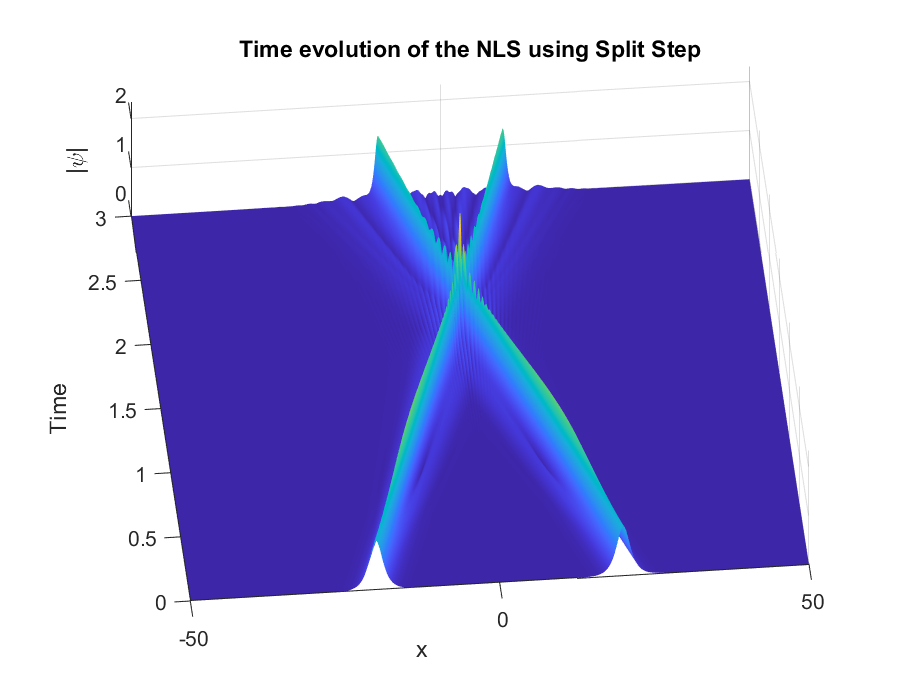
\includegraphics{Plots/splitStep_S-05}
        \caption{caption}
        \label{label}
    \end{center}
\end{figure}



\end{document}